\documentclass[12pt]{article}
\usepackage{arxiv}
\usepackage[english, russian]{babel}
\usepackage[T2A]{fontenc}
\usepackage{url}
\usepackage{booktabs}
\usepackage{nicefrac}
\usepackage{microtype}
\usepackage{lipsum}
\usepackage{graphicx}
\usepackage{natbib}
\usepackage{doi}
\usepackage{amsmath}
\usepackage{mathtools}
\usepackage{algpseudocode}
\usepackage{algorithm2e}
\usepackage{ dsfont }

%\documentclass{article}
\usepackage{array}
\usepackage{multirow}
\usepackage{wrapfig}

\usepackage{setspace}
\singlespacing % полуторный интервал для всего текста


\title{Дистилляция моделей и данных}

\author{ Баринов Никита\\
	МФТИ\\
	\And
	Филатов Андрей \\
	МФТИ       
}
\date{}

\renewcommand{\undertitle}{}
\renewcommand{\headeright}{}
\renewcommand{\shorttitle}{Дистилляция моделей и данных}

\hypersetup{
    pdftitle={Дистилляция моделей и данных},
    pdfauthor={Баринов Никита},
    pdfkeywords={Deep Learning \and Distilling the Knowledge \and Dataset Distillation}
}

\begin{document}
\maketitle

\begin{abstract}


%отдельно про дистилляцию моделей - сократить размер модели
%данных - обучить две модели можем
% не сущ-т решения одновременной 
% провели рез-ты и получили качество не сильно хуже

На сегодняшний день существует два метода дистилляции в глубоком обучении: дистилляция моделей позволяет уменьшить их размер, при этом не сильно потеряв в качестве, а дистилляция данных позволяет существенно снизить время обучения. Во всех работах эти методы рассматриваются отдельно. Поэтому провели исследование  различных комбинаций совмещения этих подходов. В результате мы выявили, что добавление дистилляции моделей при обучении дистилляции данных может значительно увеличить качество обученной модели.

% суть что мы совмещаем два подхода различным образом

    % Во многих задачах ML точность предсказания модели зависит от её размера. При этом зачастую данная зависимость выглядит достаточно тривиально: последовательное увеличение размеров модели позволяет последовательно улучшать точность её предсказаний. Но такой безграничных рост приводит к ряду проблем: существенное увеличение времени обучения, высокие требования к размерам и качеству обучающей выборки, а также вычислительные сложности. Аналогичная проблема и с данными: чем их больше, тем дольше модель на них обучается.
    % В связи с этим возникает желание одновременно <<сжать>> и данные, и модели так, чтобы на новых данных модель меньшего размера не сильно теряла в качестве. Этот процесс называется дистилляцией моделей и данных, и в статье мы предлагаем одно из решений. Вычислительные эксперименты проводятся на выборке изображений CIFAR10. 


\end{abstract}

\keywords{Deep Learning \and Distilling the Knowledge \and Dataset Distillation \and Model Compression}


\section{Введение}

Глубокое обучение добилось огромного успеха за последние несколько лет в различных областях, таких как компьютерное зрение(\cite{guo2022attention}), обработка естественного языка(\cite{raina2022natural}) и распознавание речи(\cite{subramanian2022deep}). Но всё это требует больших вычислительные и временные ресурсы. Например, как говорится в оригинальной статье \cite{radford2019language}, для обучения GPT-2 с 1.5 миллиардов параметров было использовано 40 терабайт текстовых данных, и модель обучалась на суперкомпьютерных кластерах в течение нескольких недель.

В широком диапазоне практически значимых задач машинного обучения точность предсказания модели существенно зависит от её размера. При этом зачастую данная зависимость выглядит очень просто: последовательное увеличение размеров модели позволяет последовательно улучшать точность её предсказаний. Однако такой безграничный рост приводит к ряду проблем, связанных с практическим применением итоговых моделей. Со временем начали появляться методы <<сжатия>> моделей без сильной потери качества. Появилась концепция дистилляции знаний(knowledge distillation) – это способ обучения нейросетевых моделей машинного обучения, направленный на передачу знаний от модели-учителя к модели-ученику. Первой статьёй, в которой можно встретить дистилляцию знаний в современном виде является \cite{hinton2015distilling}. В ней предлагается сжать ансамбль моделей в одну модель, тем самым значительно уменьшив её размер.

%ускорить обучение можно уменьшением выборки, но качество падает, поэтому ввели методы дист данных, кот позв создать небольшое число обучающих, на которых качество финальной модели не сильно ухудшает
Через некоторое время появляется дистилляция данных(dataset distillation) - это существенное уменьшение выборки, путём создания искусственных объектов (синтетических данных), которые агрегируют полезную информацию, хранящуюся в данных, и тем самым модель, обученная на синтетических данных будет соответствовать точности модели, обученной на полном наборе. Если мы имеем лишь несколько достаточно хорошо дистиллированных изображений, мы можем гораздо эффективнее обучить нейронную сеть на целом наборе данных, по сравнению с традиционным обучением, при котором часто используются десятки тысяч шагов градиентного спуска. Каждый элемент синтетических данных содержит в себе больше информации, чем отдельный элемент исходной выборки. 

% краткий обзор нашей по пунктам + кратко результаты
В данной работе предлагается новый подход: одновременная дистилляция модели и данных методами \cite{hinton2015distilling} и     \cite{cazenavette2022dataset}. Все эксперименты мы проводили на выборке CIFAR10. В секции \ref{41} мы провели базовый эксперимент по дистилляции моделей, в \ref{42} описано, как мы получали дистиллированные изображения, а в \ref{43} - как получали дистиллированные изображения с дистилляцией моделей, и в \ref{44} проводится главный эксперимент по совмещению двух подходов. В итоге мы выяснили, что добавление дистилляции моделей может существенно повысить качество.


\section{Обзор литературы}

 Сегодня существует несколько решений проблемы дистилляции моделей или данных в отдельности. 


% ba2014deep посмотреть
\subsection{Дистилляция моделей}
%применили дистилляцию чтобы сжать модель ансамбль в одну модель
В статье \cite{romero2014fitnets} использовали промежуточные веса или параметры слоев для обучения меньшей модели. Ещё один способ дистилляции, описанный в статье \cite{ba2014deep}, он основан на том, что меньшая модель обучается аналогично большей: она обучается
для изучения функции, которая была изучена более крупной моделью, тем самым получается конкурентоспособная производительность. В \cite{hinton2015distilling} применили дистилляцию, чтобы сжать ансамбль в одну модель. Одной из последних работ является \cite{chung2020feature}. В ней описывается дистилляция в онлайн-режиме: модель и ученик совместно оптимизируются на каждой итерации. В статье \cite{chen2021learning} описан метод: имеется граф взаимоотношений между моделями, а передача знаний осуществляется при помощи предложенной функции потерь, сохраняющей локальность.
%использовали графовые методы, чтобы перенести связи между моделью-учителеем и учеником....



%найти поновее статьи, страница 11, multi-teacher дистилл.

\subsection{Дистилляция данных}
% какую функцию они оптимизируют
В статье \cite{wang2018dataset} сначала данные инициализируются случайным шумом, а затем при помощи градиентного спуска в пространстве параметров происходит обновление синтетических данных при помощи экспертных траекторий. Описанный метод имеет явный недостаток: он ограничен числом эпох обучения. Использование теоремы о неявной функции в \cite{lorraine2020optimizing} помогает избавиться от такого недостатка. В \cite{zhao2020dataset} в качестве функции ошибки используется расстояние между градиентами этой ошибки по параметрам ученика, которые получаются при обучении на обычных и дистиллированных данных. Альтернативным вариантом может быть введение генеративной модели(может создавать новые данные, которые похожи на те, что были использованы для ее обучения), способной из шума и меток класса создавать необходимые для обучения синтетические изображения, этот подход подробно описан в \cite{such2020generative}.
Статья \cite{cazenavette2022dataset} предлагает метод дистилляции путем создания выборки, на которой динамика обучения такая же, как и на исходной.
%почему теорема о неявной функции полезна
%ванг ограничен числом эпох, а эти ограничения обошлись применением теоремы о неявной функции
%жао в кач-ве ф.ош.  исп расст....


%абстрактная вещь в начале дип лернинг чето там
%подвод к дистилляции данных, в чем прикол, позволит обечать модели намного быстрее и тд
%во многих задачах модели сильно избыточные, и для того чтобы сохранить кач-во и обобщ спос большой модели применяется подходит дистилляции моделей
% в чем вклад: предложили то то то
%в методее рассм применение, как можно примениь на релаьных задачах



\section{Постановка проблемы}

%два аргмина: модель: лосс

В этом разделе описывается формальная постановка проблем дистилляции данных, дистилляции моделей и предлагаемое решение одновременной дистилляции моделей и данных.

\subsection{Дистилляция моделей}

Введём несколько понятий:

\begin{itemize}
    \item Дистилляция модели - снижение сложности модели путем выбора модели в множестве более простых моделей на основе анализа пространства параметров и предсказаний целевой переменной более сложной фиксированной модели.

    \item Учитель - фиксированная модель, ответы которой используются при выборе модели-ученика.

    \item Ученик - модель, которая выбираемся согласно заданному критерию качества учителя.
\end{itemize}

Итак, решается задача классификации:
\[
\mathcal{D} = \{ (\mathbf{x_i}, y_i) \}_{i=1}^R,
\]
где $y_i \in \mathds{Y} = {1,2,...,R}$, $R$ - число классов, $\mathbf{x_i} \in \mathds{R}^n$.

В дистилляции Хинтона \cite{hinton2015distilling} рассматривается параметрическое семейство функций:
\[
\mathcal{G} = \{\mathbf{g} \ | \ \mathbf{g} = softmax(\mathbf{z}(\mathbf{x})/T), \ \mathbf{z}: \mathds{R}^n \rightarrow{} \mathds{R}^R\},
\eqno(1)
\]
где $\mathbf{z}$ - дифференцируемая параметрическая функция заданной структуры (нейронная сеть ученик), $T$ - параметр температуры. В качестве модели-учителя рассматривается функция $\mathbf{f}$ из множества:
\[
\mathcal{F} = \{\mathbf{f} \ | \ \mathbf{f} = softmax(\mathbf{v}(\mathbf{x})/T, \ \mathbf{v}: \mathds{R}^n \rightarrow{} \mathds{R}^R  \},
\eqno(2)
\]
где $\mathbf{v}$ - дифференцируемая параметрическая функция заданной структуры (нейронная сеть учитель), $T$ - параметр температуры. 

При этом температура $T$ имеет свойства:

\begin{enumerate} 
\item при Т $\rightarrow 0$ получаем вектор, в котором один из классов имеет единичную вероятность;
\item при Т $\rightarrow \infty$ получаем вектор, в котором все классы равновероятны.
\end{enumerate} 

Функция потерь $\mathcal{L}$ учитывает перенос информации от модели-учителя $\mathbf{f}$ к ученику $\mathbf{g}$ и имеет вид:

\[
\begin{aligned}
     \mathcal{L}(\mathbf{g,X,Y,f})=&-\sum\limits_{i=1}^{m}\sum\limits_{r=1}^{R}y_{i }^{r}\log{g^{r}(x_{i})}\bigr|_{T=1}\\
     &-\sum\limits_{i=1}^{m}\sum\limits_{r=1}^{R}f_{r}(x_{i})\bigr|_{T=T_{0} }\log{g_{r}(x_{i})}\bigr|_{T=T_{0}},
\end{aligned}
\]

где $\cdot\bigr|_{T=t}$ означает, что предыдущая функция, зависящая от $T$ берется при $T=t$ и первое слагаемое отвечает за исходную функцию потерь, а второе - за дистилляцию. Итого получаем оптимизационную задачу:
\[
\mathbf{\hat g} = \underset{\mathbf{g} \in \mathcal{G}}{\arg\min}~\mathcal{L}(\mathbf{g,X,Y,f}).
\eqno(3)
\]


\subsection{Дистилляция данных}

Пусть $\mathcal{D}_{real} = \{(\mathbf{x_i}, y_i)\}_{i = 1}^N$ --- исходная выборка. Наша задача --- создать меньшую выборку $\mathcal{D}_{syn} = \{(\mathbf{\hat x_i}, \hat y_i\}_{i = 1}^M$, где $M \ll N$ и такой, что качество модели, обученной на нём сопоставимо с качеством при обучении на исходных данных. Наш метод дистилляции предполагает создание экспертных траекторий обучения $\tau^*$, под которыми понимается последовательность параметров $\{ \theta_t^*\}_{t = 0}^T$, полученных во время обучения нейронной сети на $\mathcal{D}_{real}$. Чтобы получить экспертные траектории, предлагается обучить большое количество нейронных сетей на $\mathcal{D}_{real}$ и сохраним их параметры на каждой эпохе. Также определим $\hat\theta_t$ - параметры модели-студента, обученной на $\mathcal{D}_{syn}$ на шаге обучения $t$. На каждом шаге обучения мы будем выбирать случайно $\theta_t^*$, инициализировать этим значением параметры модели-студента $\hat\theta_t := \theta_t^*$. Установим верхнюю границу $T^{max}$ на число $t$, чтобы игнорировать ту часть обучения, где параметры меняются незначительно. 

Пусть $l(\mathcal{A}(\mathcal{D}_{syn}), \theta_t)$ - дифференцируемая функция потерь, $\mathcal{A}$ - дифференцируемая техника аугментации данных \cite{romero2014fitnets}. После инициализации параметров модели-студента мы совершим $N$ шагов градиентного спуска по параметрам $\hat\theta_t$:
\begin{equation}\label{eq1}
    \hat\theta_{t+n+1} = \hat\theta_{t+n} - \alpha\nabla l(\mathcal{A}(\mathcal{D}_{syn}), \hat\theta_{t+n}),    
\end{equation}

где $\alpha$ - шаг обучения модели-студента, используемый для обновления её параметров. 
После обучения градиентного спуска для конкретной траектории $\tau^* \in \{\tau_i^*\}$ считаем 

\begin{equation}\label{eq2}
    \mathcal{L} = \frac{\parallel\hat\theta_{t+N}-\theta_{t+M}^*\parallel_2^2}{\parallel\theta_t^* - \theta_{t+M}^* \parallel_2^2},   
\end{equation}

где $\mathcal{L}$ - функция потерь между конечными параметрами студента и учителя, нормированная на пройденное учителем расстояние, что помогает получать информацию о более поздних стадиях его обучения, где параметры меняются не сильно. В конце мы обновляем $\mathcal{D}_{syn}$ в соответствии с обучаемым параметром $\alpha$ и посчитанной функцией $\mathcal{L}$. Алгоритм \ref{alg: myalg} иллюстрирует наш метод дистилляции данных.

\RestyleAlgo{ruled}
%% This is needed if you want to add comments in
%% your algorithm with \Comment
\SetKwComment{Comment}{/* }{ */}
\begin{algorithm}[hbt!]
\caption{Data Distillation}\label{alg:two}
\KwData{$\{\tau_i^*\}$ - \text{множество параметров учителей, обученных на }$\mathcal{D}_{real}$}
\KwData{$M$ - \text{число обновлений между стартовыми и целевыми параметрами учителя}}
\KwData{$N$ - \text{число обновлений студента за один шаг дистилляции}}
\KwData{$\mathcal{A} - \text{дифференцируемая функция аугментации}$}
\KwData{$T^{max} < T - \text{максимальная стартовая эпоха}$}
\KwResult{\text{Дистиллированный набор } $\mathcal{D}_{syn}$ и $\alpha$}
$\mathcal{D}_{syn} \gets \mathcal{D}_{real}$\;
$\alpha \gets \alpha_0$\;
\For{$step : 1 \ .. \ N$}{
  $\tau^* \sim \{\tau_i^*\}, \tau^* = \{\theta_t^*\}_0^T$ - \text{выбираем траекторию обучения}\;
  $t \leq T^*$ - \text{случайно выбираем начальную эпоху}\;
  $\theta^*_t := \theta_t^*$ - \text{инициализируем веса студента параметрами учителя}\;
  \For{$n : 0 \ .. \ N-1$}{
    $b_{t+n} \sim \mathcal{D}_{syn}$ - \text{выбрать мини-батч из }$\mathcal{D}_{syn}$\;
    $\hat\theta_{t+n+1} \gets \hat\theta_{t+n} - \alpha\nabla l(\mathcal{A}(\mathcal{D}_{syn}), \hat\theta_{t+n})$\;
  }
  $\mathcal{L} \gets \parallel\hat\theta_{t+N}-\theta_{t+M}^*\parallel_2^2 / \parallel\theta_t^* - \theta_{t+M}^* \parallel_2^2$\;
  \text{Изменить } $\mathcal{D}_{syn}$ \text{ и } $\alpha$ \text{ в зависимости от } $\mathcal{L}$\;
  }
  \label{alg: myalg}
\end{algorithm}


Таким образом, оптимизационная задача, которая решает дистилляцию данных, выглядит так:
        
\begin{equation}\label{eq3}
    \mathcal{\hat D} = \underset{\mathcal{D} \in \mathcal{D}_M}{\arg\min}~ \mathcal{L}(\mathcal{D}, f, \mathcal{D}_{real}),
\end{equation}


где $\mathcal{\hat D}$ - дистиллированная выборка.



\subsection{Дистилляция моделей и данных}

Дистилляция моделей позволяет улучшить результат маленьких моделей за счет передачи знаний от большой модели к маленькой. В дистилляции данных происходит сжатие информации всей выборки в небольшой набор данных. 
% Основной подход по дистилляции данных заключается в имитации поведения модели на всех данных, за счёт синтетических данных. 
Но процедура дистилляции данных занимает долгое время и поэтому в основном используются небольшие архитектуры, чтобы ускорить процесс. Но маленькие модели не могут добиться большого качества на всех данных, но с помощью добавления дистилляции модели-учителя можно улучшить его.  В нашей работе мы предлагаем модифицированный способ дистилляции: в функцию потерь, которая используется для дистилляции данных, добавим слагаемое, отвечающее за дистилляцию знаний от модели-учителя. Тем самым, новая функция потерь будет иметь вид: 


\begin{equation}\label{eq4}
    \mathcal{L}_{new}(\mathcal{A}(\mathcal{D}_{syn}), \theta_t, \mathbf{f}, \mathbf{g}, T) = l(\mathcal{A}(\mathcal{D}_{syn}), \theta_t) - \sum\limits_{i=1}^{m}\sum\limits_{r=1}^{R}f_{r}(x_{i})\bigr|_{T=T_{0} }\log{g_{r}(x_{i})}\bigr|_{T=T_{0}},    
\end{equation}

где под $\mathbf{f}$ понимается модель-учитель, а $\mathbf{g}$ - модель, которая дистиллирует изображения. Наглядно процесс дистилляции моделей и данных изобразим на рисунке \ref{ris}.

    \begin{figure}[h!]
            \centering
            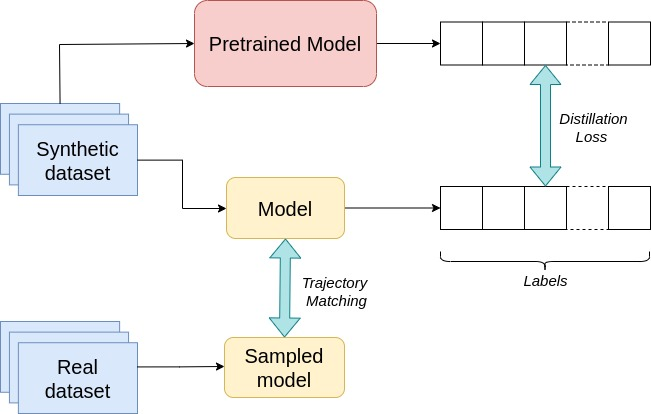
\includegraphics[width=0.5\linewidth]
            {dist.jpg}
            \caption{Одновременная дистилляция моделей и данных}
            \label{ris}
    \end{figure}

Таким образом, наша функция потерь учитывает перенос знаний от учителя к ученику, поэтому маленькие модели, которые дистиллируют изображения, должны учитывать более высокоуровневые паттерны, переданные учителем.

% Перефразировать также вывод.


% дистилляция моделей, acc на тесте mnist, описать параметры все эпохи, опт ...
% resnet50-teacher, resnet18-student. pretrained=False. torchvision.models.resnet18
% поменять число каналов на 1
% итог - две цифры два аккураси
% логгер: импорт самари райтер и во время обучения записывать в него
% таблица(-цы)
%

\section{Эксперимент}
% что такое ConvNet 
% мы обучаем да синт данных и тестируемся на тестовой выборке CIFAR10
\subsection{Дистилляция моделей}\label{41}

Проведем базовый эксперимент на выборке CIFAR10, с которым будем сравнивать результаты в дальнейшем: дистилляцию моделей. Для этого в качестве модели-учителя используем ResNet50, в качестве модели-ученика ConvNet, архитектура которой представлена в приложении \ref{pril_convnet}. Мы получили, что на ResNet50 (21.3М параметров), точность $75.28\%$, а на ConvNet (0.3М параметров) --- $73.07\%$.


Теперь используем дистилляцию моделей. Введём понятие \textit{вес дистилляции} (distillation weight) - коэффициент влияния модели-ученика. Обозначим его $\alpha$, тогда функция потерь ученика $\mathcal{L}$ примет вид:

\begin{equation}\label{eq5}
    \mathcal{L} = (1 - \alpha) \cdot H(\mathbf{f}, \mathbf{g}) + \alpha \cdot D_{KL}(\mathbf{f}|\mathbf{g}),
\end{equation}
где кросс-энтропия вычисляется по формуле:

\begin{equation}\label{eq6}
    H(\mathbf{f},\mathbf{g}) = -\sum_{x} \mathbf{f}\log \mathbf{g} ,
\end{equation}

а дивергенция Кульбака-Лейблера:

% соответствие с дист мод и перенести п и ук вверх

\begin{equation}\label{eq7}
    D_{KL}(\mathbf{f}|\mathbf{g}) = \sum_{x} \mathbf{f} \log \frac{\mathbf{f}}{\mathbf{g}} ,
\end{equation}

где $\mathbf{f}$ и $\mathbf{g}$ - предсказанные вероятности классов ученика и учителя соответственно.

% В нашем случае $D_{KL}(p|q)$ вычисляется исходя из переноса данных от модели-учителя к ученику, то есть принимает <<мягкие>> метки классов, предсказанных учителем и учеником, обозначим их $$p^*_T = softmax(\mathbf{z}(\mathbf{x})/T), \; q^*_T = softmax(\mathbf{v}(\mathbf{x})/T),$$ где $z$ и $v$ определены выше. 

Для обучения мы использовали оптимизатор SGD с шагом обучения 0.001. Мы обучали модели в течение 6 эпох. Чтобы рассмотреть работу дистилляции для различных параметров, мы провели эксперименты при $\alpha \in \{0.3, 0.7\}$, а $T\in \{0.5, 1, 2\}$.
Результаты представлены в таблице \ref{tab:table_2}.


\begin{table}[]
\begin{center}
\begin{tabular}{c|c|c}
    \hline
    \multirow{1}{*}{$T$ (температура)}& $\alpha$ (вес дистилляции)& Accuracy, \% \\
    \hline
    \multirow{2}{*}{0.5}& 0.3 & \textbf{74.84}\\
    & 0.7 & 71.72\\
    \hline
    \multirow{2}{*}{1.0}& 0.3 & \textbf{74.49}\\
    & 0.7 & 71.59\\
    \hline
    \multirow{2}{*}{2.0}& 0.3 & \textbf{75.06}\\
    & 0.7 & 71.49\\
    \hline
\end{tabular}
\end{center}
\caption{Результаты обучения ConvNet с дистилляцией от ResNet50 при различных температурах $T$ весах дистилляции $\alpha$.}
\label{tab:table_2}
\end{table}

\textbf{Вывод:} дистилляция с меньшим весом улучшило качество модели ResNet, а при дистилляции модели с большим весом, качество ухудшилось.
%обобщить вывод на веса

\subsection{Дистилляция данных}\label{42}

% На каком датасете была реализована дистилляция данных?
% Как была реализована дистилляция данных? 
% > Для дистилляции мы использовали алгоритм \ref{}.
% Какие параметры дистилляции данных использовались (Сколько эпох, траекториий и т.д.?).
% Какие архитектуры мы использовали в дистилляции данных?
% Сколько картинок на класс было синтезировано?
% Какие аугментации использовались?

Как правило, большая выборка изображений содержит избыточную для обучения информацию. Поэтому мы бы хотели сжать эти изображения в сравнительно небольшую выборку, которая синтезирует в себе основные паттерны исходной.

Итак, мы провели дистилляцию данных на выборке изображений CIFAR10. Для этого был использован алгоритм \ref{alg:two}. Для дистилляции использовались траектории обучения ConvNet на полной выборке CIFAR10: было сгенерировано 50 экспертных траекторий, каждая из которых получалась при обучении ConvNet на 60 эпох. При создании изображений использовались такие аугментации, как масштабирование, кадрирование, поворот, добавление шума.

В итоге была создана синтетическая выборка из 10 картинок на каждый из 10 классов - 100 изображений. Примеры исходных и дистиллированных изображений представлены в приложении \ref{pril_1} и \ref{pril_2}.

% #TODO Подумать,  что сделать с таблицей




% Основной эксперимент
% ResNet50 обученный на всех данных добавляется в лосс дистилляции данных. Учим ConvNet на супердистилированных данных.
% Учим ResNet50 на супердистилированных данных.
 
% СуперТаблица
% На будущее график по данным 
% интерес узнать зависимость качества от числа данных
% идеальный баланс для сжатия моделей и данных
% кажется, что когда меньше картинок на класс эффект дистилляции моделей должен быть больше


\subsection{Добавление дистилляции моделей в дистиляцию данных}\label{43}

% Зачем этот эксперимент нужен?
Когда происходит дистилляция данных, используются небольшие архитектуры, которые не могут запомнить достаточно сложные паттерны, поэтому мы решили добавить к этой процедуре дистилляцию от более сложной модели.

% соло + другие 
Теперь картинки дистиллируются и одновременно происходит дистилляция модели учителя, согласно выражению \ref{eq4}. Обозначим как $\tau$ и $\beta$ - температуру и вес дистилляции моделей при дистилляции данных. Мы использовали те же значения веса дистилляции и температуры и получили ещё 6 наборов дистиллированных изображений.
% Процесс дистилляции можно видеть на графике \ref{ris1}.

% \begin{figure}[h!]
%         \centering
%         \includegraphics[width=0.7\linewidth]
%         {dist_image.png}
%         \caption{Процесс дистилляции данных без учителя и с учителем при разных весах дистилляции и темпратурах}
%         \label{ris1}
% \end{figure}
% Как метод дистилляции моделей использовался?
% Какая модель использовалась как учитель обучении?
% Какие параметры дистилляции использовались?

% Насколько хорошо были обучены дистилированные данные и супердистилированные? 
% > Результаты обучение приведены в таблице
% > Добавить картинку для визуального сравнения
% Есть ли различие между дистилированными и супердистилированными данными на этой стадии?
% Какие дальше супердистилированные данные использовались?

% \textbf{Вывод:} на данной стадии видно, что картинки, которые получались с весом дистилляции ResNet50 0.7 давали худшее качество, чем те, которые с весом 0.3 и без учителя.

\subsection{Добавление дистилляции моделей в обучение на дистиллированных данных}\label{44}
% Зачем этот эксперимент нужен?
В этом эксперименте мы исследовали применимость дистилляции моделей при обучении на дистиллированных данных. Дистиллированные данные являются сжатым представлением целой выборки, в которой 50000 изображений, поэтому выходы модели-учителя будут релевантны, так как модель выучила глубокую структуру данных, а синтезированные данные - сжатое представление этой структуры.

Для начала, в роли базового эксперимента, мы обучили ConvNet на 50 эпох с оптимизатором SGD и кросс-энтропийной функцией потерь на картинках, полученных простой дистилляцией данных. Оценку качества модели мы производили все так же на тестовой выборке CIFAR10 (10000 изображений). Для сравнения, если мы случайным образом будем выбирать по 10 изображений из полной выборки CIFAR10 на каждый класс, то мы достигнем точности порядка \textbf{25\%}.


Мы использовали метод дистилляции моделей по Хинтону \cite{hinton2015distilling}, только теперь модель-студент(ConvNet) училась на синтетических данных и тех же аугментациях, которые использовались при их создании. В роли модели-учителя использовался ResNet50. Эксперимент был проведен при $\alpha \in \{0.3, 0.7\}$ --- вес дистилляции моделей, а $T\in \{0.5, 1, 2\}$ и всех наборах картинок, полученных ранее. 

\begin{table}[]
\begin{center}
\begin{tabular}{c|c|c}
    \hline
    \multirow{1}{*}{$\alpha$ (вес дистилляции)}& Параметры дистилляции данных & Accuracy, \%\\
    \hline
    \multirow{7}{*}{Без дистилляции}& Без учителя & \textbf{37.42}\\
                        & $\beta = 0.3$, $\tau=0.5$ & 29.68\\
                        & $\beta = 0.3$, $\tau=1$ & 23.58\\
                        & $\beta = 0.3$, $\tau=2$ & 29.65\\
                        & $\beta = 0.7$, $\tau=0.5$ & 20.98\\
                        & $\beta = 0.7$, $\tau=1$ & 32.57\\
                        & $\beta = 0.7$, $\tau=2$ & 16.72\\
                        
    \hline
    \multirow{4}{*}{0.3}& Без учителя & \textbf{41.18}\\
                        & $\beta = 0.3$, $\tau=0.5$ & 30.59\\
                        & $\beta = 0.7$, $\tau=1$ & 35.33\\
                        & $\beta = 0.3$, $\tau=2$ & 29.18\\
    \hline
    \multirow{4}{*}{0.7}& Без учителя & \textbf{42.88}\\
                        & $\beta = 0.3$, $\tau=0.5$ & 34.33\\
                        & $\beta = 0.7$, $\tau=1$ & 39.61\\
                        & $\beta = 0.3$, $\tau=2$ & 38.05\\
    \hline
\end{tabular}
\end{center}
\caption{Результаты при дистилляции ResNet50 на ConvNet, обучаемый на дистиллированных изображениях при различных температурах $T$ весах дистилляции $\alpha$.}
\label{tab:table_4}
\end{table}

Для сравнения мы обучили ConvNet на семи наборах дистиллированных изображений: без учителя и шесть при всех комбинациях $\alpha$ и $T$. Обучение производилось в 50 эпох, использовался оптимизатор SGD и кросс-энтропийная функция потерь. Результаты представлены в таблице \ref{tab:table_4}, где $\beta$ и $\tau$ - параметры, которые определяют влияние модели-учителя на дистилляцию данных.
% Как метод дистилляции моделей использовался?
% Какая модель использовалась как учитель обучении?
% Какие параметры дистилляции использовались?

% Какие различие в результатах? Есть ли прирост в данных?
% Почему есть такой буст?


% добавить сравнение со 100 рандомными
% \beta \tau как параметры дистилляции данных
% \begin{table}[]
% \begin{center}
% \begin{tabular}{c|c}
%     \hline
%     Параметры дистилляции данных & Accuracy, \% \\
%     \hline
%     Без учителя & 33.89 $\pm 1.23\%$ \\
%     \hline
%     $\alpha = 0.3$, $T=2$ & $29.65 \pm 0.89\% $\\
%     \hline
%     $\alpha = 0.3$, $T=1$ & $23.58 \pm 1.09\%$ \\
%     \hline
%     $\alpha = 0.3$, $T=0.5$ & $29.68 \pm 1.21\%$ \\
%     \hline
%     $\alpha = 0.7$, $T=2$ & $16.72 \pm 1.47\%$\\
%     \hline
%     $\alpha = 0.7$, $T=1$ & $32.57 \pm 0.98\%$ \\
%     \hline
%     $\alpha = 0.7$, $T=0.5$ & $20.98 \pm 1.05\%$ \\
%     \hline
% \end{tabular}
% \end{center}
% \caption{Зависимость Accuracy при обучении ConvNet на дистиллированных изображениях.}
% \label{tab:table_3}
% \end{table}

% \begin{table}[]
% \begin{center}
% \begin{tabular}{c|c|c}
%     \hline
%     \multirow{1}{*}{$\tau$}& $\beta$ & Accuracy, \% \\
%     \hline
%     \multirow{2}{*}{0.5}& 0.3 & \textbf{29.68}\\
%     & 0.7 & 20.98\\
%     \hline
%     \multirow{2}{*}{1.0}& 0.3 & 23.58\\
%     & 0.7 & \textbf{32.57}\\
%     \hline
%     \multirow{2}{*}{2.0}& 0.3 & \textbf{29.65}\\
%     & 0.7 & 16.72\\
%     \hline
% \end{tabular}
% \end{center}
% \caption{Зависимость Accuracy при обучении ConvNet на дистиллированных изображениях.}
% \label{tab:table_3}
% \end{table}

Мы сразу заметили, что на трех наборах изображений результат значительно хуже, чем на остальных, поэтому мы решили рассмотреть влияние дистилляции моделей для оставшихся четырех наборов. Мы добавили дистилляцию моделей с температурой $T = 0.5$, использовали функцию потерь \ref{eq5}, оптимизатор SGD и 50 эпох обучения. Результаты можно видеть в таблице \ref{tab:table_4}. 

% сделать разделение по \beta и \tau
% выделить лучшие результаты в секции


\textbf{Вывод:} мы видим существенное различие в результатах при добавлении дистилляции моделей: при обучении с дистилляцией качество выросло на 3-5\%. 
% использование другой модели дает буст

%\subsection{Дистилляции моделей на дистиллированных данных}
% Зачем это эксперимент?
% > Предыдущий эксперимент показал эффективность применения дистилляции моделей, которые обучены на всех данных. В этом эксперименты мы решили происследовать применимость дистилляции моделей, когда модель учитель была обучена на дистилированных данных.

% Как метод дистилляции моделей использовался?
% Какая модель использовалась как учитель обучении?
% Какие параметры дистилляции использовались?

% Какой итог?


\section{Вывод}

В этой работе мы проанализировали различные подходы к дистилляции моделей и данных, создали алгоритм дистилляции данных с использованием дистилляции моделей. 
% добавление дист мод помогает
% преимущества
В результате мы выяснили, что дистилляция моделей действительно помогает при обучении на синтетической выборке и это имеет свои преимущества, такие как более качественные дистиллированные изображения за счет использования модели-учителя.

В дальнейшем мы хотим проверить это на более крупных и сложных выборках, на задачах распознавания текста и звука, и использовать другие методы дистилляции.
% Что мы проанализировали в этой работе?
% Какие результаты анализа?
% Какие дальнейшее продолжения работы?
% другие методы дист мод и данных, провести более масштабные эксперименты


\newpage
\bibliographystyle{unsrt}
\bibliography{ref}

\newpage
\section{Приложение}

    \begin{figure}[h!]
            \centering
            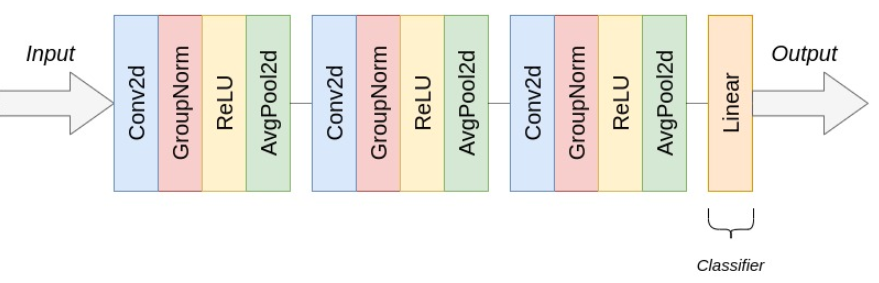
\includegraphics[width=0.55\linewidth]
            {convnet_foto1.png}
            \caption{Архитектура ConvNet}
            \label{pril_convnet}
    \end{figure}

    \begin{figure}[h!]
            \centering
            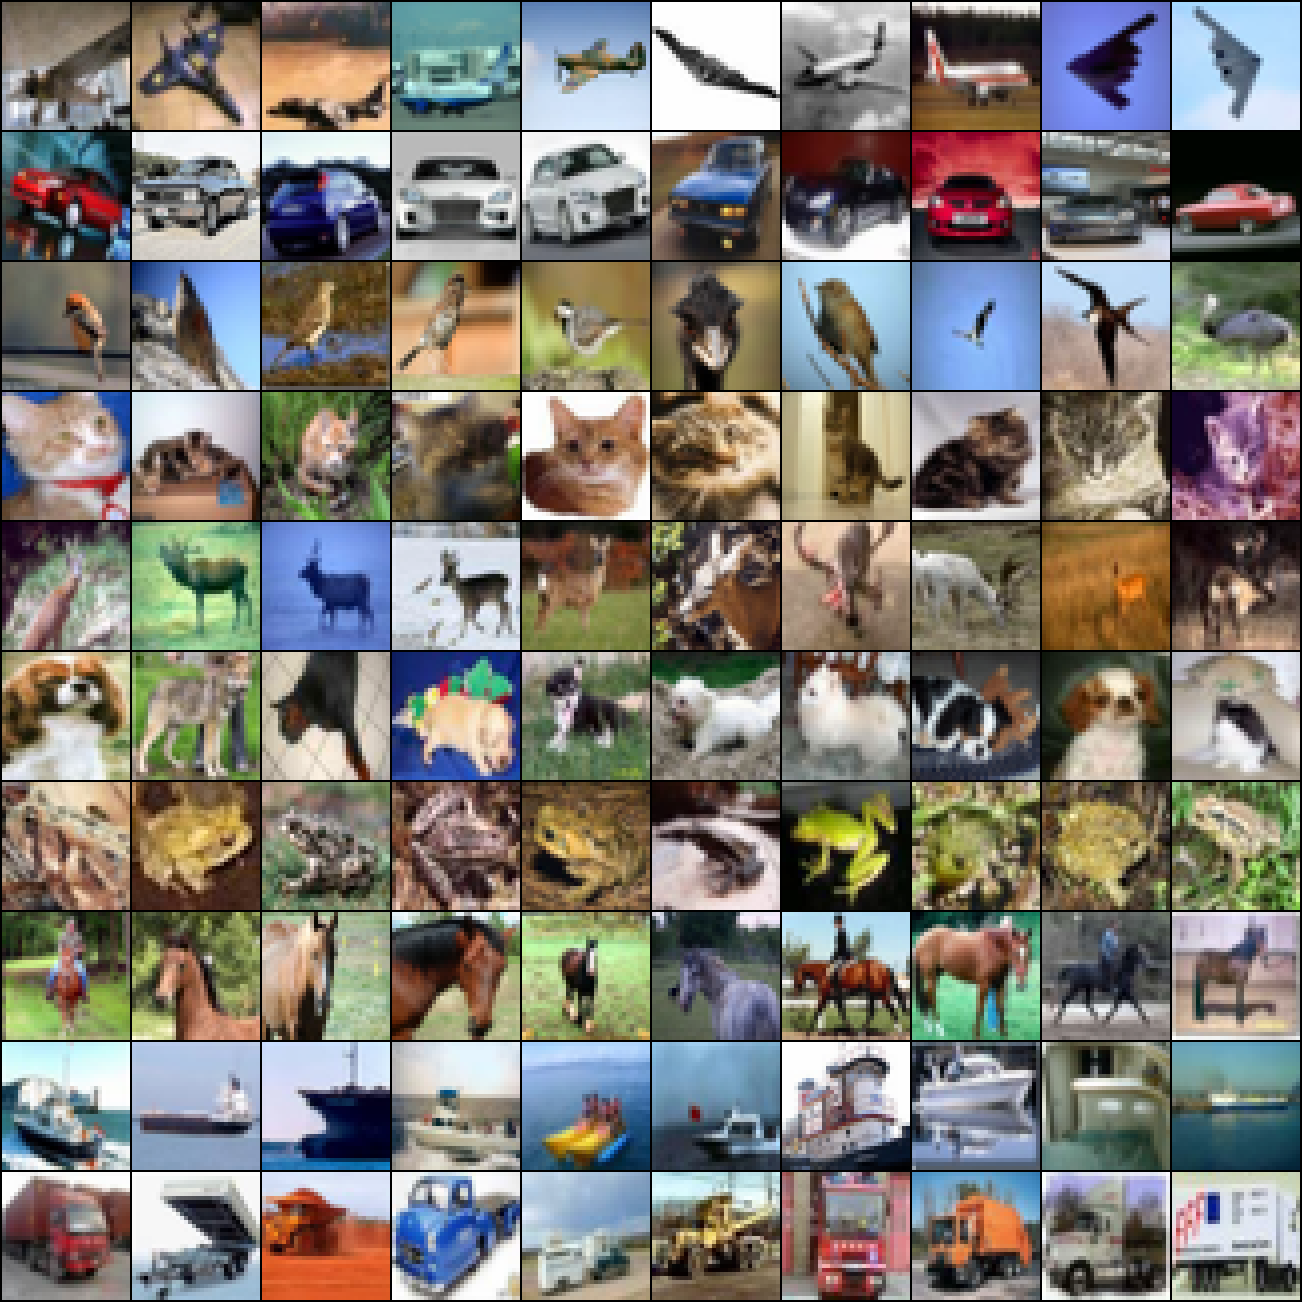
\includegraphics[width=0.55\linewidth]
            {reconst_solo.png}
            \caption{Исходные изображения из CIFAR10 по 10 на класс}
            \label{pril_1}
    \end{figure}
    
    \begin{figure}[h!]
            \centering
            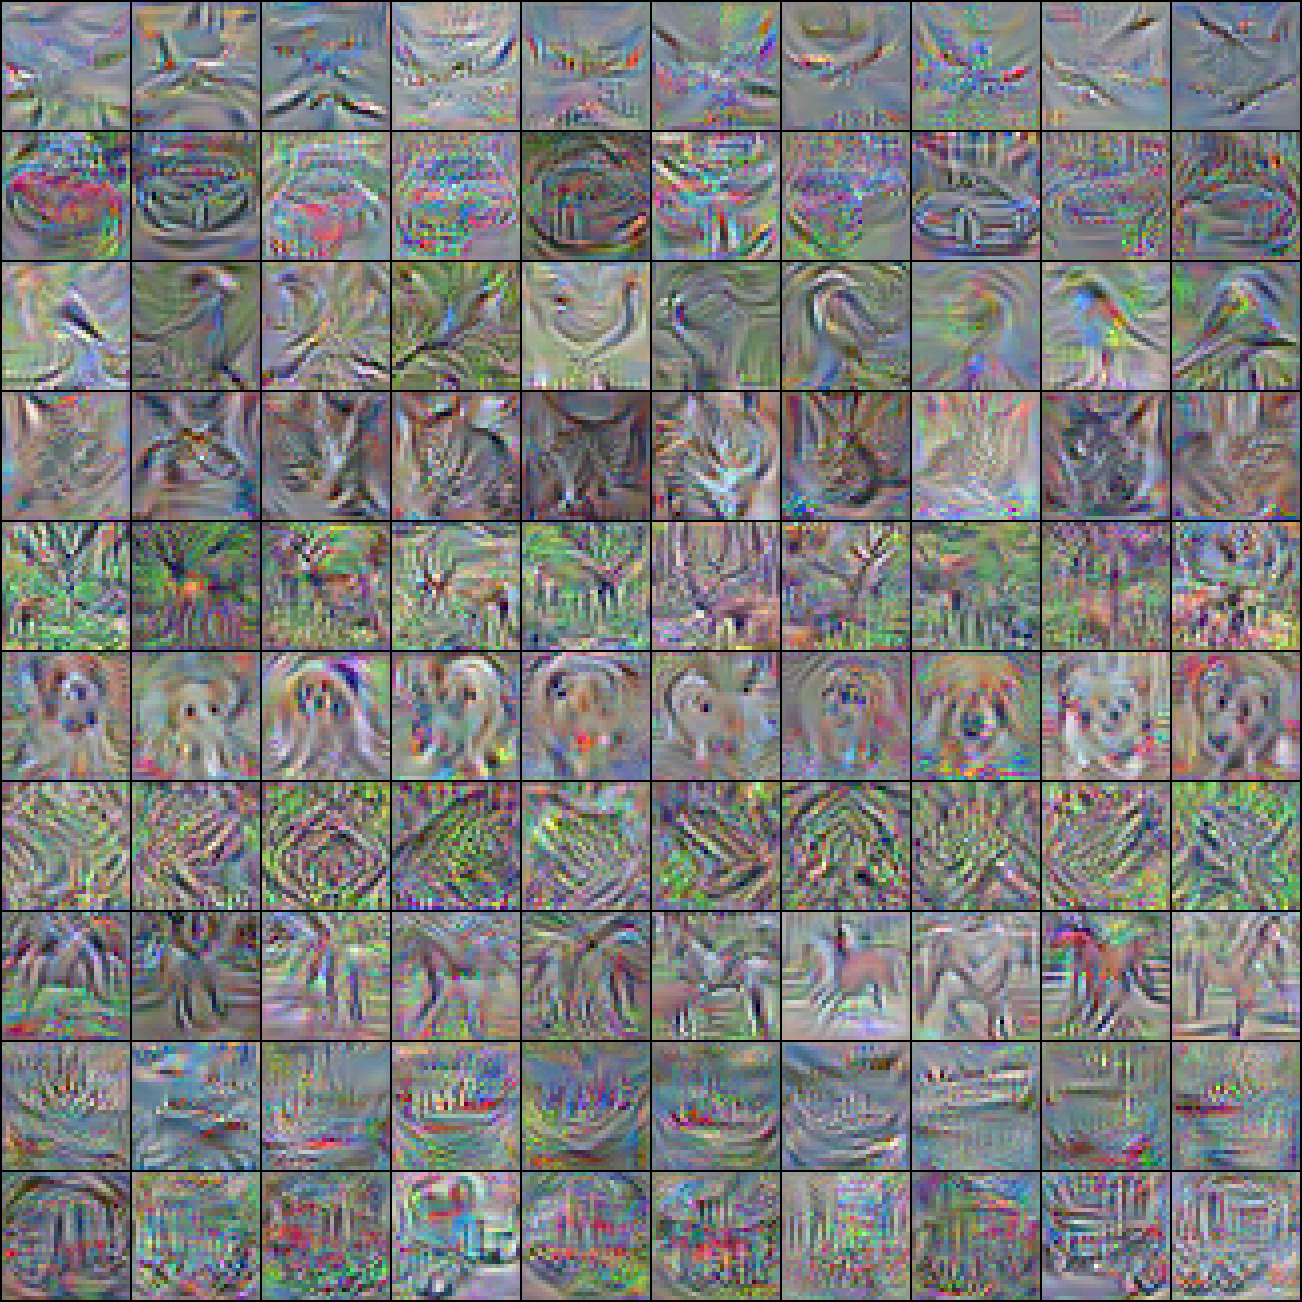
\includegraphics[width=0.55\linewidth]
            {dist_solo.png}
            \caption{Дистиллированные изображения из CIFAR10 по 10 на класс}
            \label{pril_2}
    \end{figure}

\begin{figure}[ht] \label{fig7} 
  \begin{minipage}[b]{0.5\linewidth}
    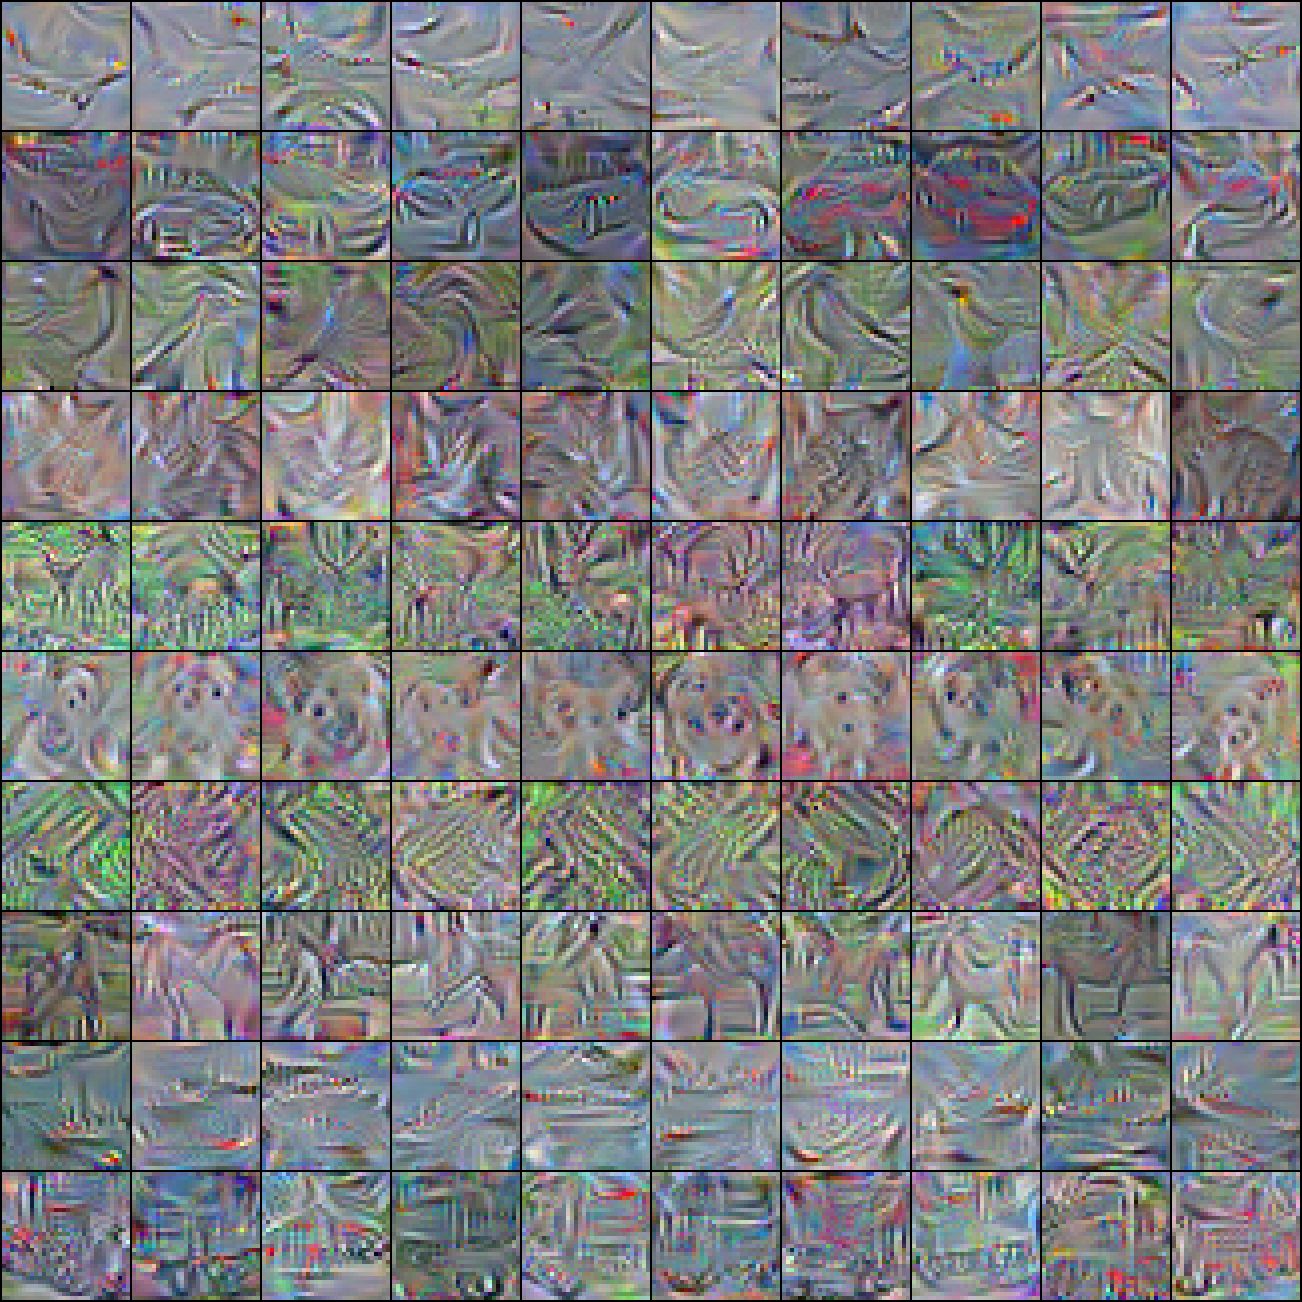
\includegraphics[width=1\textwidth]{dist_2_03.png}
    \caption{\centeringДистилляция изображений с весом \;\;\;учителя $\alpha = 0.3$ и $T = 2$} 
  \end{minipage} 
  \begin{minipage}[b]{0.5\linewidth}
    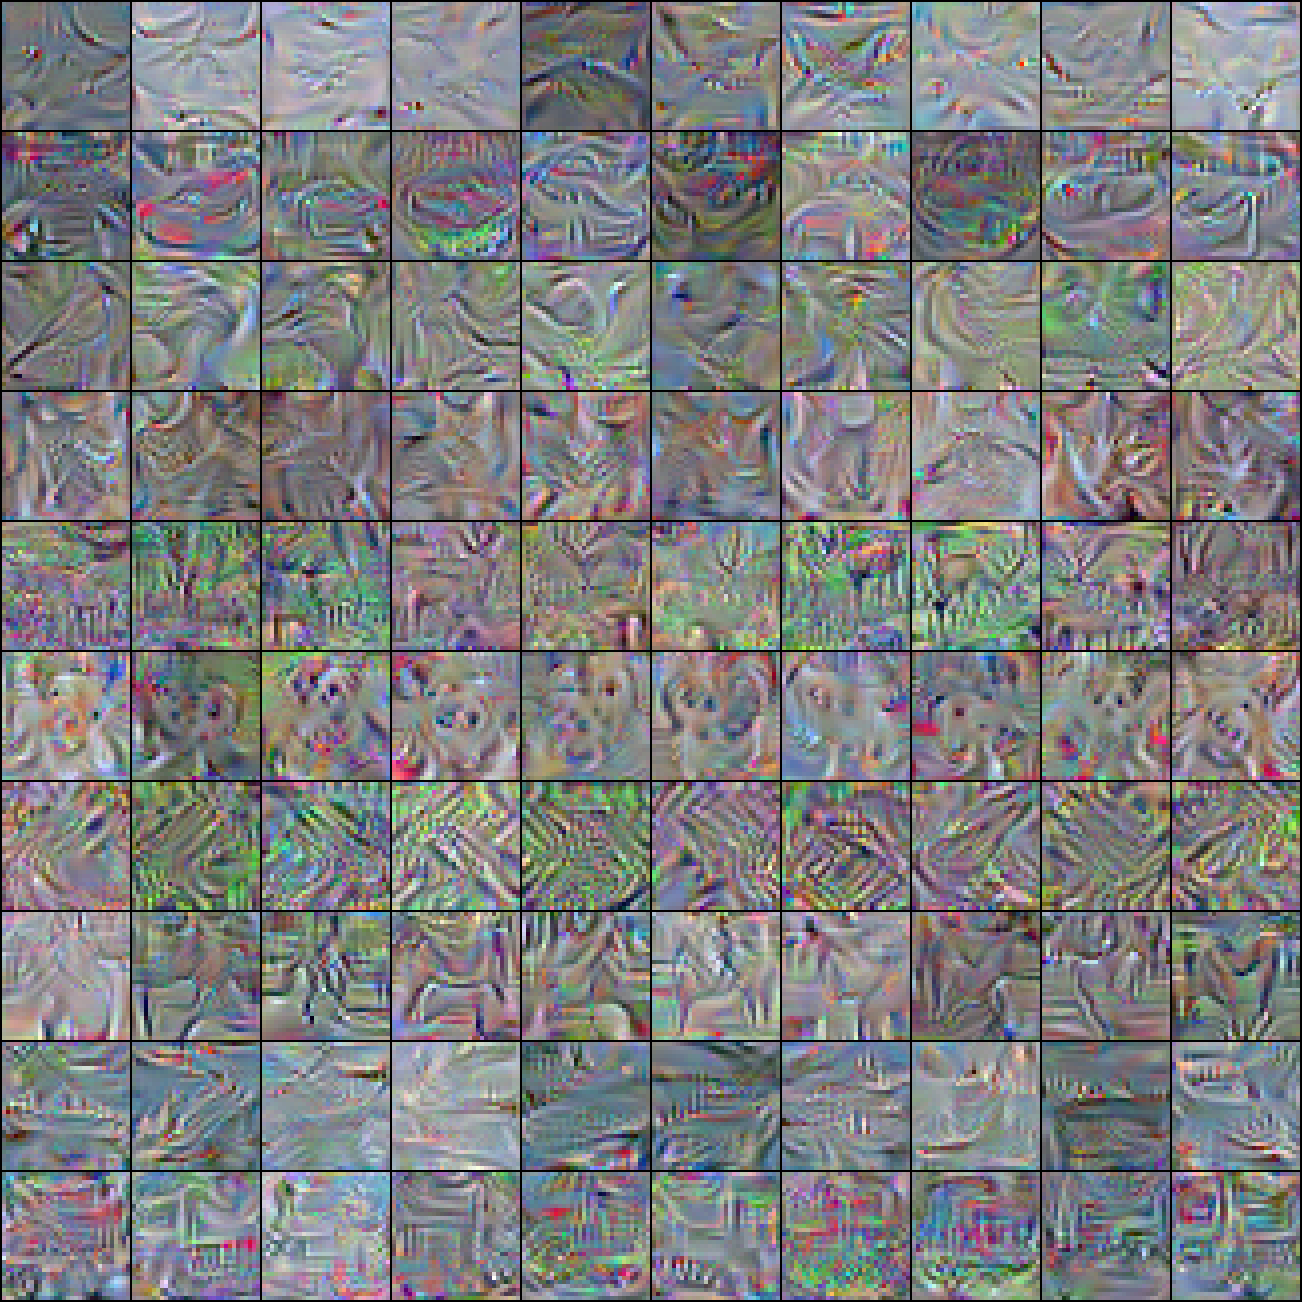
\includegraphics[width=1\textwidth]{dist_05_07.png}
    \caption{\centeringДистилляция изображений с весом \;\;\;учителя $\alpha = 0.7$ и $T = 0.5$} 
  \end{minipage} 
\end{figure}
    

\end{document}